\documentclass[a4paper, 11pt]{article}

\usepackage[top=112pt, bottom=112pt, left=90pt, right=85pt]{geometry}
\usepackage{geometry, amssymb, csquotes, amsmath, graphicx, mathtools, amsthm, calc, accents} 
\usepackage[hidelinks]{hyperref}
\usepackage[utf8]{inputenc}
\usepackage{xcolor}
\usepackage{todonotes}
%\usepackage{parskip}

\newcommand{\rem}[2][noinline]{\todo[#1, color=gray!20!white,size=\footnotesize]{\texttt{Rem}: #2}}
\newcommand{\doubletilde}[1]{\tilde{\raisebox{0pt}[0.85\height]{$\tilde{#1}$}}}
\newcommand{\tripletilde}[1]{\tilde{\raisebox{0pt}[0.85\height]{$\doubletilde{#1}$}}}

\newtheorem{prop}{Proposition}
\newtheorem{definition}{Definition}
\newtheorem{lemma}{Lemma}
\newtheorem{theor}{Theorem}
\newtheorem{cor}{Corollary}
\newtheorem{conjecture}{Conjecture}

\DeclareMathOperator\artanh{artanh}
\DeclareMathOperator\tr{tr}

\hypersetup{
  urlcolor = black,
  citecolor = black,
  pdftitle = {notes},
  pdfsubject = {notes},
  pdfpagemode = UseNone
}

% \hypersetup{
%     colorlinks=true,
%     linkcolor=blue,
%     filecolor=magenta,      
%     urlcolor=blue,
% }

\newcommand\underl[2]{\mathrel{\mathop{#2}\limits_{#1}}}

\title{\textbf{Finding moments from master equation}}
\date{\today}
\begin{document}
\maketitle

\begin{abstract}
  Here we discuss the exact ways of finding the moments of the probability distribution directly from the {\it master equation} (ME). The main method is to perturbatively find the asymptotic expansion (at least to the second order) of the {\it generating function}, which is directly related to the moments of the probability distribution. First we demonstrate the method on simple examples, then we derive the expressions (4,5,6) from \cite{PAULSSON2005157}, and then attempt to apply the method to the simple neuron models \textcolor{red}{(in progress)}. Note that the method gives the exact expressions for the moments, which is demonstrated for the simple examples by finding the generating function exactly.
\end{abstract}

\tableofcontents

\section{Introduction}
Often the probability distribution arises as a solution to the maser equation, and here we show how to find the moments of the unknown distribution without actually finding the distribution itself.
\subsection{The problem}

The master equation (ME) from \cite{PAULSSON2005157} reads as
\begin{equation} \label{full_Paulsson_ME}
  \begin{split} 
    \frac{dP_{n_1,n_2,n_3}(t)}{dt} = &\lambda_1^+\left[(N_1-n_1+1)P_{n_1-1,n_2,n_3}(t) - (N_1-n_1)P_{n_1,n_2,n_3}(t)\right]\\
    + & \lambda_1^-\left[(n_1+1)P_{n_1+1,n_2,n_3}(t) - n_1P_{n_1,n_2,n_3}(t)\right] \\
    + & \lambda_2\left[n_1P_{n_1,n_2-1,n_3}(t) - n_1P_{n_1,n_2,n_3}(t)\right]\\
    + & \tau_2^{-1}\left[(n_2+1)P_{n_1,n_2+1,n_3}(t) - n_2P_{n_1,n_2,n_3}(t)\right]\\
    + & \lambda_3\left[n_2P_{n_1,n_2,n_3-1}(t) - n_2P_{n_1,n_2,n_3}(t)\right]\\
    + & \tau_3^{-1}\left[(n_3+1)P_{n_1,n_2,n_3+1}(t) - n_3P_{n_1,n_2,n_3}(t)\right]
  \end{split}
\end{equation}
and takes into account activation/deactivation of $N_1$ independent copies of the same gene ($n_1$ is the number of active replicas of the gene at any given time), mRNA production and decay ($n_2$ is the number of mRNA molecules), and the production and decay of proteins ($n_3$ is the number of proteins).

In this introductory section we will show how to find the means, variances and correlations of all variables ${n_1, n_2, n_3}$ from the  probability distribution satisfying the equation (\ref{full_Paulsson_ME}) at stationarity\footnote{Note that the method is not limited to stationarity.}. Before that, we will demonstrate the method on two simple examples which are, in fact, identical, but we solve them differently to demonstrate the issues that arise from not embedding all the information to the master equation (which reduces dimensionality).

\subsection{Independent gene switching} \label{sec::independent_gene_switching}
\rem[inline]{I dont see very well what is the jump process in this case. A very natural way to describe a jump process is to give its infinitesimal generator $\mathbf A$ which is somehow the adjoint of the Fokker Planck equation. Formally, $\mathbf Af(x) = \lim\limits_{\delta\to 0}(E_x(f(X_\delta))-x)/\delta$
	
In your case, I'd say that \[(\mathbf Ah)(n) = \lambda_1^+1_{n<N_1}\left(f(n+1)-f(n)\right) + \lambda_1^-1_{n>0}\left(f(n-1)-f(n)\right) \]}
We will now demonstrate the approach by solving the problem of independent switching of $N_1$ gene replicas, for which the master equation is given by\footnote{Compare with the first two lines of (\ref{full_Paulsson_ME}).}
\begin{equation} \label{gene_switching_ME}
  \begin{split} 
    \frac{dP_{n_1}(t)}{dt} = &\lambda_1^+\left[(N_1-n_1+1)P_{n_1-1}(t) - (N_1-n_1)P_{n_1}(t)\right]\\
    + & \lambda_1^-\left[(n_1+1)P_{n_1+1}(t) - n_1P_{n_1}(t)\right],
  \end{split}
\end{equation}
where $n_1$ is the number of active genes.

The generating function of the distribution $P_{n_1}(t)$ is defined as
\begin{equation} \label{gen_func_def} 
  G(z_1; t) = \sum_{n_1=0}^{\infty}P_{n_1}(t)z_1^{n_1}.
\end{equation}
Note that the moments of the probability distribution $P_{n_1}$ can be found from the derivatives of the generating function with respect to the corresponding variables, i.e.
\begin{align}
  \frac{\partial G(z_1; t)}{\partial z_1}\bigg\rvert_{z_1=1} &= \sum_{n_1=0}^{\infty} n_1P_{n_1}(t) = \langle n_1\rangle(t); \label{1st_der_of_GF}\\
  \frac{\partial^2 G(z_1; t)}{\partial z_1^2}\bigg\rvert_{z_1=1} &= \sum_{n_1=0}^{\infty} n_1(n_1-1)P_{n_1}(t) = \langle n_1\rangle^2(t) - \langle n_1\rangle(t)\label{2nd_der_of_GF}.
\end{align}

The generating function allows recasting the master equation (\ref{gene_switching_ME}) in a PDE form as follows. First, we multiply both sides of the ME (\ref{gene_switching_ME}) by $z_1^{n_1}$ and sum over $n_1$, which gives
\begin{equation*}
  \begin{split}
    \sum_{n_1=0}^{\infty}\frac{dP_{n_1}(t)}{dt}z_1^{n_1} = &\lambda_1^+\sum_{n_1=0}^{\infty}\left[(N_1-n_1+1)P_{n_1-1}(t) - (N_1-n_1)P_{n_1}(t)\right]z_1^{n_1}\\
    + & \lambda_1^-\sum_{n_1=0}^{\infty}\left[(n_1+1)P_{n_1+1}(t) - n_1P_{n_1}(t)\right]z_1^{n_1}.
  \end{split}
\end{equation*}
Then, using the definition of the generating function (\ref{gen_func_def}) and the following identities
\begin{align*}
  & \sum_{n_1=0}^{\infty}P_{n_1-1}(t)z_1^{n_1} = z_1\sum_{n_1=0}^{\infty}P_{n_1-1}(t)z_1^{n_1-1} = z_1G(z_1;t);\\
  & \sum_{n_1=0}^{\infty}P_{n_1+1}(t)z_1^{n_1} = \frac{1}{z_1}\sum_{n_1=0}^{\infty}P_{n_1+1}(t)z_1^{n_1+1} = \frac{1}{z_1}G(z_1;t);\\
  & \sum_{n_1=0}^{\infty}n_1P_{n_1}(t)z_1^{n_1} = z_1\frac{\partial}{\partial z_1}\sum_{n_1=0}^{\infty}P_{n_1}(t)z_1^{n_1} = z_1\frac{\partial G(z_1; t)}{\partial z_1};\\
  & \sum_{n_1=0}^{\infty}n_1P_{n_1-1}(t)z_1^{n_1} = z_1\frac{\partial}{\partial z_1}\sum_{n_1=0}^{\infty}P_{n_1-1}(t)z_1^{n_1} = z_1\frac{\partial}{\partial z_1} \left(z_1G(z_1; t)\right);\\
  & \sum_{n_1=0}^{\infty}n_1P_{n_1+1}(t)z_1^{n_1} = z_1\frac{\partial}{\partial z_1}\sum_{n_1=0}^{\infty}P_{n_1+1}(t)z_1^{n_1} = z_1\frac{\partial}{\partial z_1} \left(\frac{1}{z_1}G(z_1; t)\right),
\end{align*}
we recast the equation (\ref{gene_switching_ME}) in the form of the following first-order partial differential equation (PDE)
\begin{equation*} \label{gene_switching_PDE}
  \frac{\partial G(z_1;t)}{\partial t} + (\lambda_1^+z_1 + \lambda_1^-)(z_1-1)\frac{\partial G(z_1;t)}{\partial z_1} = \lambda_1^+N_1(z_1-1)G(z_1;t),
\end{equation*}
which can be solved using the method of characteristics.

\subsubsection{Finding the generating function exactly}
For convenience we introduce new variable as
\begin{equation*}
  x_1 := z_1 - 1
\end{equation*}
and denote
\begin{equation*}
  \mathcal G(x_1; t) = G(z_1(x_1); t).
\end{equation*}
in terms of which the PDE (\ref{gene_switching_PDE}) becomes
\begin{equation} \label{gene_switching_PDE_x}
  \frac{\partial \mathcal G(x_1;t)}{\partial t} + (\lambda_1^+x_1 + \frac{1}{\tau_1})x_1\frac{\partial \mathcal G(x_1;t)}{\partial x_1} = \lambda_1^+N_1x_1\mathcal G(x_1;t),
\end{equation}
where $\tau_1 := (\lambda_1^+ + \lambda_1^-)^{-1}$.
The characteristic equations for the nonhomogeneous quasilinear PDE (\ref{gene_switching_PDE}) are given by
\begin{equation*}
  \begin{dcases}
    \dot t = \tau;\\
    \dot x_1 = \lambda_1^+x_1^2 + \frac{1}{\tau_1}x_1;\\
    \dot{\mathcal G} = \lambda_1^+N_1x_1\mathcal G,
  \end{dcases}
\end{equation*}
which have the following {\it first integrals}
\begin{align*}
  C_1& = -\left(P_\text{on}+\frac{1}{x_1}\right)\mathrm e^{t/\tau_1}\\
  C_2& = \left(\frac{-\mathrm e^{t/\tau_1}}{x_1P_{on}}\right)^{N_1}\mathcal G,
\end{align*}
where
\begin{equation*}
  P_\text{on} = \frac{\lambda_1^+}{\lambda_1^+ + \lambda_1^-} = \lambda_1^+\tau_1.
\end{equation*}

The general solution is given by\footnote{As an exercise one can check this solution by direct substitution to (\ref{gene_switching_PDE_x}).}
\begin{equation}\label{n1_general_solution}
  \mathcal G(x_1;t) = \left(-x_1P_{\text{on}}\mathrm e^{-t/\tau_1}\right)^{N_1}f\left(\left(P_{on}+\frac{1}{x_1}\right)\mathrm e^{t/\tau_1}\right),
\end{equation}
where $f(.)$ is an arbitrary function defined by the initial conditions.

Assuming that the initial number of active genes was $m$, i.e.
\begin{equation}\label{initial_condition}
  P_{n_1}(t=0) = \delta_{n_1,m} \implies \mathcal G(x_1; t=0) = (x_1+1)^m,
\end{equation}
we arrive to
\begin{equation*}
  f(\xi) = \left(\frac{\xi - P_\text{on}}{-P_{\text{on}}}\right)^{N_1}\cdot\left(\frac{1+\xi-P_\text{on}}{\xi-P_{\text{on}}}\right)^m,
\end{equation*}
from which (\ref{n1_general_solution}) reads as\footnote{Which, of course, can also be checked by the direct substitution to the PDE (\ref{gene_switching_PDE_x}) and the initial condition (\ref{initial_condition}).}
\begin{equation}\label{n1_special_solution}
  \mathcal G(x_1; t) = \left(x_1P_\text{on}\left(1-\mathrm e^{-t/\tau_1}\right)+1\right)^{N_1}\cdot\left(\frac{x_1\mathrm e^{-t/\tau_1}}{x_1P_\text{on}\left(1-\mathrm e^{-t/\tau_1}\right)+1} + 1\right)^m.
\end{equation}

%% \begin{equation}
%%   \mathcal G(x_1; t) = \left(x_1P_{\text{on}}\left(1-\mathrm e^{-t/\tau_1}\right)\right),
%% \end{equation}
%% and finally

Note that, as any generating function, $\mathcal G(x_1=0; t)=1$, and from (\ref{n1_special_solution}) it is clear that
\begin{equation}\label{binomial_gen_function}
  \lim_{t\to\infty}\mathcal G(x_1; t) = \left(1 + x_1P_\text{on}\right)^{N_1},
\end{equation}
which is expected, since (\ref{binomial_gen_function}) is the generating function of the binomial distribution with the probability of success $P_\text{on}$.

\subsubsection{Asymptotic expansion of the stationary solution} \label{switching_asymptotic_expansion}
Unfortunately, it is rarely possible to find the generating function exactly, but since the moments of the probability distribution only depend on the behaviour of $\mathcal G(x_1;t)$ in the vicinity of $x_1=0$, they can be obtained by means of an asymptotic expansion of $\mathcal G(x_1;t)$ around this point. In this section we exemplify this method on the model above, whose exact solution can be used for verification. To do this we substitute the function $\mathcal G$ in the form of its asymptotic expansion at $x_1=0$
\begin{equation}\label{two_compartment_hopping_expansion}
  \mathcal G(x_1;t) = 1 + \mathcal G^{(1)}(t)x_1 + \frac{1}{2}\mathcal G^{(2)}(t) x_1^2 + ... = 1 + \langle n_1\rangle(t) x_1 + \left[\langle n_1^2 \rangle(t)-\langle n_1\rangle(t)\right]x_1^2 + ...
\end{equation}
to the equation (\ref{gene_switching_PDE_x}), which at stationarity reads as
\begin{equation*}
  (\lambda_1^+x_1 + \frac{1}{\tau_1})x_1\frac{d\mathcal G(x_1)}{dx_1} = \lambda_1^+N_1x_1\mathcal G(x_1),
\end{equation*}
or equivalently
\begin{equation*}
  (P_{\text{on}}x_1 + 1)x_1\frac{d\mathcal G(x_1)}{dx_1} = P_{\text{on}}N_1x_1\mathcal G(x_1).
\end{equation*}
This substitution leads to
\begin{equation*}
  \left(P_{\text{on}}-\frac{1}{2}P_{\text{on}}N_1\right)\mathcal G^{(2)}x_1^3 + \left(\mathcal G^{(2)} + \mathcal G^{(1)}P_{\text{on}} - P_{\text{on}}N_1G^{(1)}\right)x_1^2 + \left(G^{(1)}-P_{\text{on}}N_1\right)x_1 = 0,
\end{equation*}
where the $\mathcal O(x^3)$ terms must be ignored, since we only do the expansion up to the second order. The unknown coefficients $\{\mathcal G^{(i)}\}$ are found by voiding all consecutive orders in $x$ up to two, which gives a non-degenerate system of two linear equations for two unknowns
\begin{equation*}
  \begin{dcases}
    G^{(1)}-P_{\text{on}}N_1 = 0\\
    \mathcal G^{(2)} - \mathcal G^{(1)}P_{\text{on}}(N_1-1) = 0,
  \end{dcases}
\end{equation*}
from which
\begin{equation*}
  \mathcal G^{(1)} = P_{\text{on}}N_1; \qquad     \mathcal G^{(2)} = P_{\text{on}}^2N_1(N_1-1).
\end{equation*}
Noticing that, as clear from (\ref{1st_der_of_GF}), (\ref{2nd_der_of_GF}) and the expansion (\ref{two_compartment_hopping_expansion}),
\begin{equation*}
  \mathcal G^{(1)} = \langle n_1 \rangle; \qquad \mathcal G^{(2)} = \langle n_1^2 \rangle - \langle n_1 \rangle,
\end{equation*}
the mean is found to be
\begin{equation*}
  \langle n_1\rangle = P_{\text{on}}N_1,
\end{equation*}
and the variance $\sigma^2 = \langle n_1^2 \rangle - \langle n_1 \rangle^2$ is given by
\begin{equation*}
  \sigma^2 = \mathcal G^{(2)} + \mathcal G^{(1)} - {\mathcal G^{(1)}}^2 = P_{\text{on}}^2N_1(N_1-1) + P_{\text{on}}N_1 - P_{\text{on}}^2N_1^2 = N_1P_{\text{on}}(1-P_{\text{on}}),
\end{equation*}
which are the mean and the variance of a binomial distribution with the success probability $P_{\text{on}}$ and $N_1$ trials. Note that these results are fully consistent with (\ref{binomial_gen_function}).

\subsection{Hopping between compartments}
We will now consider the problem of hopping between two spatial compartments, which is mathematically equivalent to the problem from Section \ref{sec::independent_gene_switching}, but we will approach it differently. Suppose the number of molecules in one compartment (say, soma) is $m_0$, and in another (say, dendrite) is $m_1$. The events of hopping are independent, and the ME for the process is given by
\begin{equation*}
  \begin{split}
    \frac{dP_{m_0, m_1}(t)}{dt} = &\nu^+\left[(m_0+1)P_{m_0+1,m_1-1}(t)-m_0P_{m_0,m_1}(t)\right]\\ + &\nu^-\left[(m_1+1)P_{m_0-1, m_1+1}(t) - m_1P_{m_0, m_1}(t)\right].
  \end{split}
\end{equation*}

\subsection{Finding the generating function exactly}
The corresponding PDE for the generating function is given by
\begin{equation}\label{hopping_PDE}
  \frac{\partial\mathcal G(\mathbf x; t)}{\partial t} + \nu^+(x_0-x_1)\frac{\partial\mathcal G(\mathbf x; t)}{\partial x_0} + \nu^-(x_1-x_0)\frac{\partial\mathcal G(\mathbf x; t)}{\partial x_1} = 0,
\end{equation}
which we solve using the method of characteristics.

The general solution of the PDE (\ref{hopping_PDE}) is given by
\begin{equation*}
  \mathcal G(\mathbf x; t) = f\left((x_0-x_1)\mathrm e^{-(\nu^-+\nu^+)t}, x_0\nu^-+\nu^+x_1\right),
\end{equation*}
where $f(.,.)$ is an arbitrary function of two arguments defined by the initial conditions.

If we assume that the total number of molecules is given by $M$ and at $t=0$ there was $n$ proteins in the soma (i.e. $M-n$ molecules in the dendrite), the initial probability distribution reads as
\begin{equation*}
  P_{m_0, m_1}(t=0) = \delta_{n,m_0}\delta_{M-n,m_1},
\end{equation*}
which has the following generating function
\begin{equation}\label{hopping_init_cond}
  \mathcal G(\mathbf x; t=0) = (x_0+1)^n(x_1+1)^{M-n}.
\end{equation}

The solution of the PDE (\ref{hopping_PDE}) with the initial condition (\ref{hopping_init_cond}) is given by
\begin{equation*}
  \begin{split}
    \mathcal G(\mathbf x; t) = &\left[x_0+1+P_{on}\left(1-\mathrm e^{-\frac{t}{\tau}}(x_1-x_0)\right)\right]^n\\
    &\cdot\left[x_0+1+(x_1-x_0)\left(P_{on}+\mathrm e^{-\frac{t}{\tau}}(1-P_{on})\right)\right]^{M-n},
  \end{split}
\end{equation*}
where $\tau := (\nu^++\nu^-)^{-1}$ and $P_{on} = \nu^+\tau$.
\subsection{Asymptotic expansion of the stationary solution}
In this section we will provide a simple example of finding the first two moments of a probability distribution satisfying a master equation by asymptotic expansion of $\mathcal G(\mathbf x; t)$ in the vicinity of $\mathbf x = \mathbf 0$ in multidimensional case.
\begin{equation*}
  \mathcal G(\mathbf x; t)\underl{x\to 0}{=} \boldsymbol{\mathcal G}^{(1)}(t)\mathbf x + \frac{1}{2}\mathbf x^T\boldsymbol{\mathcal G}^{(2)}(t)\mathbf x + \mathcal O(|\mathbf x|^3),
\end{equation*}
where
\begin{equation*}
  \boldsymbol{\mathcal G}^{(1)}(t) =
  \begin{pmatrix}
    \langle m_0\rangle\ 
    \langle m_1 \rangle
  \end{pmatrix}
\end{equation*}
is the gradient, while
\begin{equation*}
  \boldsymbol{\mathcal G}^{(2)}(t) =
  \left( \begin{array}{cc}
    \langle m_0^2 \rangle - \langle m_0\rangle & \langle m_0m_1\rangle\\
    \langle m_0m_1\rangle & \langle m_0^2 \rangle - \langle m_0\rangle \\
  \end{array} \right)
\end{equation*}
is the Hessian of $\mathcal G(\mathbf x; t)$ at $\mathbf x = \mathbf 0$.

Substitution to the PDE (\ref{hopping_PDE}) gives the following equation in the first order
\begin{equation*}
  \nu^+(x_0-x_1)\mathcal G_0^{(1)} + \nu^-(x_1-x_0)\mathcal G_1^{(1)}=0,
\end{equation*}
which, after collecting the coefficients of $x_1$ and $x_0$ leads to the degenerate system of two linear equations for two unknowns
\begin{equation*}
  \begin{dcases}
    \nu^+\mathcal G_0^{(1)} - \nu^-\mathcal G_1^{(1)} = 0\\
    -\nu^+\mathcal G_0^{(1)} + \nu^-\mathcal G_1^{(1)} = 0,
  \end{dcases}
\end{equation*}
from which
\begin{equation*}
  \mathcal G_1^{(1)} = \frac{\nu^+}{\nu^-}\mathcal G_0^{(1)}.
\end{equation*}

The identity for the second order is given by
\begin{equation*}
  \nu^+(x_0^2-x_1x_0)\mathcal G^{(2)}_{00} + \nu^+(x_0x_1-x_1^2)\mathcal G_{01}^{(2)}+\nu^-(x_1^2-x_0x_1)\mathcal G_{11}^{(2)} + \nu^-(x_1x_0-x_0^2)\mathcal G_{01}^{(2)} = 0,
\end{equation*}
which leads to the following degenerate system of three linear equations for the two unknowns
\begin{equation*}
  \begin{dcases}
    \nu^+\mathcal G_{00} - \nu^-\mathcal G_{01} = 0\\
    -\nu^+\mathcal G_{00} + \nu^+\mathcal G_{01} - \nu^-G_{11} + \nu^-\mathcal G_{01} = 0\\
    \nu^+\mathcal G_{01} + \nu^-\mathcal G_{11} = 0.
  \end{dcases}
\end{equation*}

This degeneracy leads to the two free parameters ($\alpha$ and $\beta$) in the expansion
\begin{equation*}
  \mathcal G(\mathbf x; t) \underl{t\to\infty}{=}\alpha
  \begin{pmatrix}
    \nu^-\ 
    \nu^+
  \end{pmatrix}
  \begin{pmatrix}
  x_0\\
  x_1
  \end{pmatrix}
  + \frac{\beta}{2}\mathbf x^T
  \left( \begin{array}{cc}
    {\nu^-}^2 & \nu^+\nu^-\\
    \nu^+\nu^- & {\nu^+}^2 \\
  \end{array} \right)\mathbf x
  + \mathcal O(|\mathbf x|^3),
\end{equation*}
and comes from the fact that, unlike Section \ref{switching_asymptotic_expansion}, the coefficients from different orders do not mix up. The compartment hopping problem is, however, fully equivalent to that in Section \ref{switching_asymptotic_expansion} and to resolve the ambiguity in $\boldsymbol{\mathbf G}^{(1)}$ and $\boldsymbol{\mathbf G}^{(2)}$ we need to provide an extra information that $m_0+m_1=M$, which is implicitly embedded\footnote{It is this information that allows reducing the dimensionality of the problem.} to the model from Section \ref{sec::independent_gene_switching}. The ambiguity in the first order terms is resolved by enforcing
\begin{equation*}
  \langle m_0 \rangle + \langle m_1\rangle = \alpha\nu^- + \alpha\nu^+ = M \implies \alpha = M\tau,
\end{equation*}
where $\tau = (\nu^- + \nu^+)^{-1}$, and in the second order
\begin{equation*}
  \langle(m_0 + m_1)^2\rangle = \langle m_0^2\rangle + \langle m_1^2\rangle + 2\langle m_0m_1\rangle = M^2, 
\end{equation*}
from which
\begin{equation*}
  \langle m_0^2\rangle - \langle m_0\rangle + \langle m_1^2\rangle - \langle m_1\rangle + 2\langle m_0m_1\rangle = \left(\mathcal G_{00}^{(2)} + \mathcal G_{11}^{(2)} + 2\mathcal G_{01}^{(2)} \right) = M^2 - M\tau\nu^- - M\tau\nu^-, 
\end{equation*}
and finally
\begin{equation*}
  \beta\left({\nu^-}^2 + {\nu^+}^2 + 2\nu^-\nu^+\right) = M(M-1),
\end{equation*}
from where
\begin{equation*}
  \beta = M(M-1)\tau^2.
\end{equation*}

Finally we arrive to the following asymptotic expansion 
\begin{equation*}
  \mathcal G(\mathbf x; t) \underl{t\to\infty}{=}M\tau
  \begin{pmatrix}
    \nu^-\ 
    \nu^+
  \end{pmatrix}
  \begin{pmatrix}
  x_0\\
  x_1
  \end{pmatrix}
  + \frac{M(M-1)}{2}\tau^2\mathbf x^T
  \left( \begin{array}{cc}
    {\nu^-}^2 & \nu^+\nu^-\\
    \nu^+\nu^- & {\nu^+}^2 \\
  \end{array} \right)\mathbf x
  + \mathcal O(|\mathbf x|^3).
\end{equation*}

\subsection{Master equation from \cite{PAULSSON2005157}}
Using the method as we did in Section \ref{sec::independent_gene_switching}, the PDE for the generating function is found to be
\begin{equation*}
  \begin{split}
    &\frac{\partial G}{\partial t} + \left[\lambda_1^+z_1(z_1-1) + \lambda_1^-(z_1-1) - \lambda_2(z_2-1)z_1\right]\frac{\partial G}{\partial z_1}\\ &+ \left[\frac{1}{\tau_2}(z_2-1) - \lambda_3(z_3-1)z_2\right]\frac{\partial G}{\partial z_2} + \frac{1}{\tau_3}(z_3-1)\frac{\partial G}{\partial z_3} = \lambda_1^+N_1(z_1-1)G,
  \end{split}
\end{equation*}
or, in terms of $\mathbf x = \mathbf z - \mathbf 1$ and $\mathcal G$
\begin{equation} \label{full_Paulsson_PDE_x}
  \begin{split}
    & \frac{\partial \mathcal G}{\partial t} + \left[(\lambda_1^+x_1+\frac{1}{\tau_1})x_1  - \lambda_2x_2(x_1+1)\right]\frac{\partial \mathcal G}{\partial x_1}\\ &+ \left[\frac{1}{\tau_2}x_2 - \lambda_3x_3(x_2+1)\right]\frac{\partial \mathcal G}{\partial x_2} + \frac{1}{\tau_3}x_3\frac{\partial \mathcal G}{\partial x_3} = \lambda_1^+N_1x_1\mathcal G,
  \end{split}
\end{equation}
where $\tau_1 = (\lambda_1^+ + \lambda_1^-)^{-1}$.

Characteristic equations are given by
\begin{equation} \label{full_characteristics}
  \begin{dcases}
    \dot t = 1\\
    \dot x_1 = \lambda_1^+(x_1+1)x_1 + \lambda_1^-x_1 - \lambda_2x_2(x_1+1)\\
    \dot x_2 = \frac{1}{\tau_2}x_2 - \lambda_3x_3(x_2+1)\\
    \dot x_3 = \frac{1}{\tau_3}x_3\\
    \dot {\mathcal G} = \lambda_1^+N_1x_1\mathcal G
  \end{dcases}
\end{equation}
and we need to find its first integrals $\{C_i(\mathbf x; t; \mathcal G)|i=1,2,3,4\}$.

After using the first characteristic equation and setting $t = \xi$ (where $\xi$ is the parameter of the characteristics) the system of ODEs (\ref{full_characteristics}) can be approached by solving the 4-th ODE for $x_3$, which gives
\begin{equation*}
  x_3 = C_1\mathrm e^{t/\tau_3} \left(\implies C_1(\mathbf x; t; \mathcal G) = x_3e^{-t/\tau_3}\right),
\end{equation*}
then substituting the result into the ODE for $x_2$, which gives
\begin{equation*}
  \begin{split}
    x_2 = -\lambda_3C_1\exp\left(\frac{t}{\tau_2}-\lambda_3C_1\tau_3\mathrm e^{t/\tau_3}\right)\int\exp\left[t\left(\frac{1}{\tau_3} - \frac{1}{\tau_2}\right) + \lambda_3C_1\tau_3\mathrm e^{t/\tau_3}\right]dt\\ + C_2\exp\left(\frac{t}{\tau_2}-\lambda_3C_1\tau_3\mathrm e^{t/\tau_3}\right)
  \end{split}
\end{equation*}
then solving the second ODE for $x_1$, and then substituting $x_1$ to the last characteristic equation, which can be solved by separation.

Unfortunately, it seems that the expressions are too complicated to obtain the first integrals in a manageable way. Therefore, we need some simplifications/approximations.

\subsection{Asymptotic expansion of the stationary solution}
Substitution of the second-order expansion to the PDE (\ref{full_Paulsson_PDE_x}) gives
\begin{equation*}
  \begin{split}
    \left(\lambda_1^+x_1^2-\lambda_2x_1x_2+\frac{1}{\tau_1}x_1-\lambda_2x_2\right)\left({\mathcal G}_1 + {\mathcal G}_{11}x_1 + {\mathcal G}_{12}x_2 + {\mathcal G}_{13}x_3\right)\\
    + \left(-\lambda_3x_2x_3 + \frac{1}{\tau_2}x_2 - \lambda_3x_3\right)\left({\mathcal G}_2 + {\mathcal G}_{21}x_1 + {\mathcal G}_{22}x_2 + {\mathcal G}_{23}x_3\right)\\
    +\frac{1}{\tau_3}x_3\left({\mathcal G}_3 + {\mathcal G}_{31}x_1 + {\mathcal G}_{32}x_2 + {\mathcal G}_{33}x_3\right) = \lambda_1^+N_1x_1\left(1 + {\mathcal G}_1x_1 + {\mathcal G}_2x_2 + {\mathcal G}_3x_3\right),
  \end{split}
\end{equation*}
which in the first order in $|x|$ reads as
\begin{equation*}
  \frac{1}{\tau_1}\mathcal G_1x_1 - \mathcal G_1\lambda_2x_2 + \frac{1}{\tau_2}\mathcal G_2x_2 - \lambda_3\mathcal G_2x_3 + \frac{1}{\tau_3}\mathcal G_3x_3 - \lambda_1^+N_1x_1 = 0,
\end{equation*}
which leads to
\begin{align*}
  \frac{1}{\tau_1}{\mathcal G}_1 = \lambda_1^+N_1\implies&\langle n_1\rangle = {\mathcal G}_1 = \lambda_1^+\tau_1N_1 = P_{on}N_1\\
  {\mathcal G}_1\lambda_2 = \frac{1}{\tau_2}{\mathcal G}_2\implies &\langle n_2\rangle = {\mathcal G}_2=\lambda_2\tau_2{\mathcal G}_1 = \lambda_2\tau_2P_{on}N_1\\
  {\mathcal G}_2\lambda_3 = \frac{1}{\tau_3}{\mathcal G}_3 \implies &\langle n_3\rangle = {\mathcal G}_3 = \lambda_3\tau_3{\mathcal G}_2 = \lambda_3\tau_3\lambda_2\tau_2P_{on}N_1
\end{align*}
The second order gives
\begin{equation*}
  \begin{split}
    \left(\frac{1}{\tau_1}{\mathcal G}_{11} - \lambda_1^+{\mathcal G}_1\left(N_1-1\right)\right)x_1^2
    +\left(\frac{1}{\tau_2}{\mathcal G}_{22} - \lambda_2{\mathcal G}_{12}\right)x_2^2
    + \left(\frac{1}{\tau_3}{\mathcal G_{33}}-\lambda_3{\mathcal G_{23}}\right)x_3^2\\
    + \left(\frac{\tau_1+\tau_2}{\tau_1\tau_2}{\mathcal G}_{12} - \lambda_2{\mathcal G}_{11} - \lambda_2{\mathcal G}_1 - \lambda_1^+N_1{\mathcal G}_2\right)x_1x_2
    + \left(\frac{\tau_1+\tau_3}{\tau_1\tau_3}{\mathcal G}_{31} - \lambda_3{\mathcal G}_{21} - \lambda_1^+N_1{\mathcal G}_3\right)x_1x_3\\
    + \left(\frac{\tau_2+\tau_3}{\tau_2\tau_3}{\mathcal G}_{23} - \lambda_2{\mathcal G}_{13} - \lambda_3{\mathcal G}_{22} - \lambda_3{\mathcal G}_2\right)x_2x_3 = 0,
  \end{split}
\end{equation*}
which leads to the nondegenerate system of six linear equations for six independent components of $\boldsymbol{\mathcal G}^{(2)}$, which are found to be
\begin{align}
      {\mathcal G}_{11}& = P_{\text{on}}^2N_1(N_1-1) \label{G_11_Paulsson}\\
      {\mathcal G}_{12}& = \frac{\tau_1}{\tau_1+\tau_2}\tau_2\lambda_2P_{\text{on}}N_1\left[P_{\text{on}}\left(N_1-1\right)+\lambda_1^+N_1\tau_2+1\right]\\
      {\mathcal G}_{22}& = \frac{\tau_1}{\tau_1+\tau_2}(\tau_2\lambda_2)^2P_{\text{on}}N_1\left[P_{\taxt{on}}(N_1-1)+\lambda_1^+N_1\tau_2+1\right] \label{G_22_Paulsson} \\
      {\mathcal G}_{13}& = \frac{\tau_1}{\tau_1+\tau_3}\lambda_2\tau_2\lambda_3\tau_3P_{\text{on}}N_1\left[\lambda_1^+N_1\tau_3 + \frac{\tau_1}{\tau_1+\tau_2}\left(N_1(\lambda_1^+\tau_2+P_{\text{on}})+1-P_{\text{on}}\right)\right]\\
      \begin{split}
        {\mathcal G}_{23}& = \frac{\tau_2}{\tau_2+\tau_3}\tau_3\lambda_3\tau_2\lambda_2P_{\text{on}}N_1\Bigg[1 + \frac{\tau_1\tau_2\lambda_2}{\tau_1+\tau_2}\left(P_{\text{on}}(N_1-1)+\lambda_1^+N_1\tau_2+1\right)\\& + \lambda_2\frac{\tau_1\tau_3}{\tau_1+\tau_3}\left(\lambda_1^+N_1\tau_3 + \frac{\tau_1}{\tau_1+\tau_2}\left(N_1(\lambda_1^+\tau_2+P_{\text{on}})+1-P_{\text{on}}\right)\right)\Bigg]
      \end{split}\\
      \begin{split}
        {\mathcal G}_{33}& = \frac{\tau_2}{\tau_2+\tau_3}(\tau_3\lambda_3)^2\tau_2\lambda_2P_{\text{on}}N_1\Bigg[1 + \frac{\tau_1\tau_2\lambda_2}{\tau_1+\tau_2}\left(P_{\text{on}}(N_1-1)+\lambda_1^+N_1\tau_2+1\right)\\& + \lambda_2\frac{\tau_1\tau_3}{\tau_1+\tau_3}\left(\lambda_1^+N_1\tau_3 + \frac{\tau_1}{\tau_1+\tau_2}\left(N_1(\lambda_1^+\tau_2+P_{\text{on}})+1-P_{\text{on}}\right)\right)\Bigg] \label{G_33_Paulsson}
      \end{split}
\end{align}
Note from the following expression for the variance
\begin{equation}\label{sigma2_from_G}
  \sigma_i^2 = {\mathcal G}_{ii} + {\mathcal G}_i - {\mathcal G}_i^2
\end{equation}
and (\ref{G_11_Paulsson}) it is clear that
\begin{equation*}
  \frac{\sigma_1^2}{\langle n_1\rangle^2} = \frac{1-P_{\text{on}}}{\langle n_1\rangle},
\end{equation*}
which is the expression (6) from \cite{PAULSSON2005157}. Similarly, using (\ref{G_22_Paulsson}) and (\ref{sigma2_from_G}) it is easy to show that
\begin{equation*}
  \frac{\sigma_2^2}{\langle n_2\rangle^2} = \frac{1}{\langle n_2\rangle} + \frac{1-P_{\text{on}}}{\langle n_1\rangle}\frac{\tau_1}{\tau_1+\tau_2},
\end{equation*}
which is the expression (5) from \cite{PAULSSON2005157}. The expression (4) from \cite{PAULSSON2005157}, which reads as
\begin{equation*}
  \frac{\sigma_3^2}{\langle n_3\rangle^2} = \frac{1}{\langle n_3\rangle} + \frac{1}{\langle n_2\rangle}\frac{\tau_2}{\tau_2+\tau_3} + \frac{1-P_{\text{on}}}{\langle n_1\rangle}\frac{\tau_2}{\tau_2+\tau_3}\frac{\tau_1}{\tau_1+\tau_3}\frac{\tau_1+\tau_3+\tau_1\tau_3/\tau_2}{\tau_1+\tau_2},
\end{equation*}
can be obtained similarly using (\ref{G_33_Paulsson}) and (\ref{sigma2_from_G}).

\section{The simple neuron model}
\subsection{Notation}
In this section we will adopt the following notation.
\begin{center}
  \begin{tabular}{|c|c|}
    \hline
        {\bf Symbol}         &{\bf Meaning}\\ \hline
        $n$                 &Number of active gene replicas \\ \hline
        $N$                 &Total number of gene replicas \\ \hline
        $m_i$               &Number of mRNA in the $i$-th compartment \\ \hline
        $M$                 &Total number of mRNAs\\ \hline
        $l_i$               &Number of free proteins in the $i$-th compartment\\ \hline
        $L$                 &Total number of proteins\\ \hline
        $q_{ij}$            &Number of proteins bound to $j$-th synapse of $i$-th dendrite\\ \hline
        $\mathbf s$        &The complete state of the system, i.e. $\{n, \mathbf m,\mathbf l, \mathbf q\}$\\ \hline
        $\lambda_1^+$        &Rate of gene activation\\ \hline
        $\lambda_1^-$        &Rate of gene deactivation\\ \hline
        $\tau_1$           &$\tau_1 = (\lambda_1^+ + \lambda_1^-)^{-1}$\\ \hline
        $\lambda_2$        &Rate of mRNA synthesis\\ \hline
        $\tau_2$           &mRNA lifetime (same for all compartments)\\ \hline
        $\kappa_i$          &Rate of protein synthesis in $i$-th compartment\\ \hline
        $\tau_3$          &Protein lifetime (same for all compartments)\\ \hline
        $\nu_{ij}$         &Rate of mRNA hopping from compartment $i$ to compartment $j$ \\ \hline
        $\theta_{ij}$      &Rate of protein hopping from compartment $i$ to compartment $j$ \\ \hline
        $\eta_{ij}$        &Rate of protein binding to $j$-th synapse on $i$-th dendrite \\ \hline
        $\gamma_{ij}$        &Rate of protein unbinding from $j$-th synapse on $i$-th dendrite \\ \hline
        $D$                 &Total number of dendrites \\ \hline
  \end{tabular}
\end{center}

In this model mRNAs and free (not bound to the synapses) proteins hop between the compartments and disintegrate over time.

In what follows we will denote the probability of state $\mathbf s$ at time $t$ as $P_{\mathbf s}(t)$. The notation $P^{\mathbf s}_{m+1}(t)$ should be understood as the probability of state $\mathbf s$ with increased by one number of mRNAs\footnote{This notation makes expressions a lot shorter, but care is needed to keep the letters as they are given in the table, i.e. $m$ for mRNAs, $p$ for proteins etc.}. Similarly, $P^{\mathbf s}_{q_{ij}-1, p_i+1}(t)$ is the probability of a state $\mathbf s$ at time $t$ with decreased by one number of proteins bound to the $j$-th synapse of $i$-th dendrite and increased by one number of free proteins in $i$-th dendrite.

%% It turns out to be convenient to parametrise the numbers of mRNAs in the compartments as $\{M,m_1,m_2,...\}$, and the number of mRNAs in the soma $m_0$ can be easily obtained from this parametrisation as $m_0=M-m_1-m_2-...-m_D$. Same for the free proteins.


\subsection{The simplest model of neuron}
\begin{figure}
  \begin{center}
    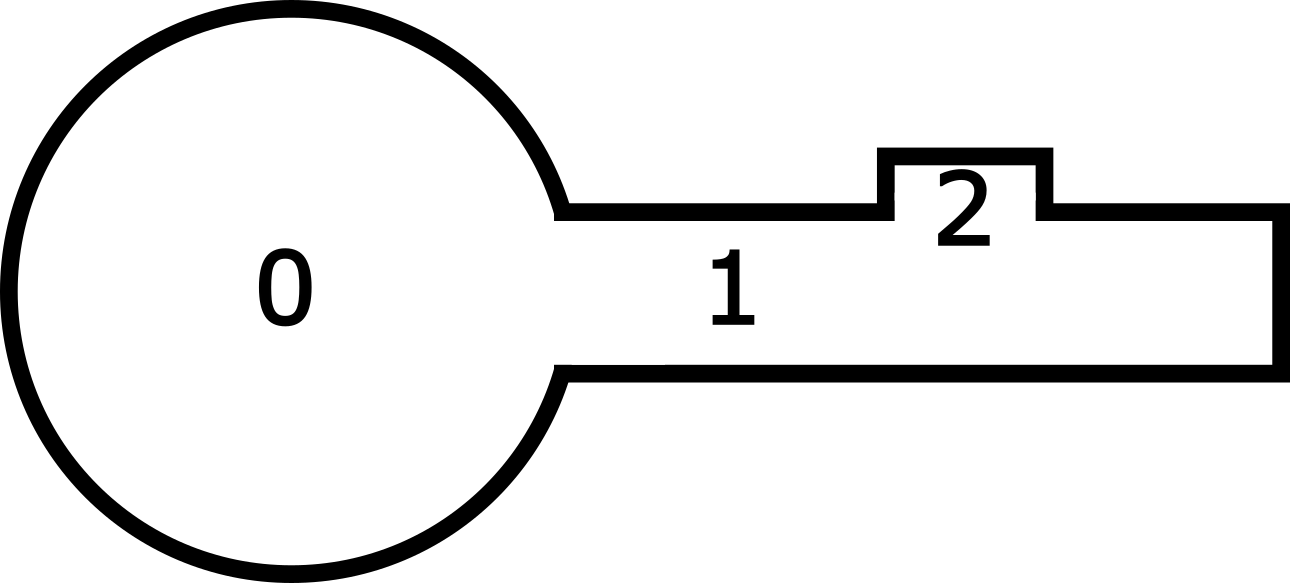
\includegraphics[width=7cm]{img/simplest_neuron.png}
  \end{center}  
  \caption{The simplest (of its kind) model of a neuron with two spatial compartments soma (``$0$'') and unbranched dendrite (``$1$'') with a single synapse (``$2$''). Transcription happens in the soma, while mRNAs and proteins travel between the soma and dendrite degrading over time. Proteins can bind to or unbind from the synapse. Proteins bound to the synapse do not decay.}
  \label{50_node_triad_sample}
\end{figure}
In this section we attempt to find the means and the variances of the protein counts in the simplest possible model of neuron of our kind.

\subsubsection{Master equation}
The model should capture the following:
\begin{enumerate}
\item \textcolor{red}{Gene activation/deactivation};
\item \textcolor{green}{mRNA production (only in the soma) and degradation (in both compartments)};
\item \textcolor{blue}{mRNA hopping};
\item \textcolor{brown}{Free protein production (in both compartments) and degradation (in both compartments, but not in the synapse)};
\item \textcolor{cyan}{Free protein hopping};
\item \textcolor{pink}{Protein binding/unbinding from the synapse}.
\end{enumerate}
The master equation that captures these processes reads as
\begin{equation*}
  \begin{split}
    \frac{dP_{\mathbf s}(t)}{dt} &= \textcolor{red}{\lambda_1^+\left[\left(N-n+1\right)P_{n-1}^{\mathbf s}(t) - \left(N-n\right)P_{\mathbf s}(t)\right] + \lambda_1^-\left[(n+1)P^{\mathbf s}_{n+1}(t) - nP_{\mathbf s}(t)\right]}\\
    & \textcolor{green}{+ \lambda_2n\left[P^{\mathbf s}_{m_0-1}(t) - P_{\mathbf s}(t)\right] + \frac{1}{\tau_2}\left[(m_0+1)P^{\mathbf s}_{m_0+1}(t) - m_0P_{\mathbf s}(t)\right]}\\ &\textcolor{green}{+ \frac{1}{\tau_2}\left[(m_1+1)P^{\mathbf s}_{m_1+1}(t) - m_1P_{\mathbf s}(t)\right]} \textcolor{blue}{+ \nu_{01}\left[(m_0+1)P^{\mathbf s}_{m_0+1,m_1-1}(t) - m_0P_{\mathbf s}(t)\right]}\\
    &\textcolor{blue}{+ \nu_{10}\left[(m_1+1)P^{\mathbf s}_{m_0-1,m_1+1}(t) - m_1P_{\mathbf s}(t)\right]} \textcolor{brown}{+ \kappa_0m_0\left[P^{\mathbf s}_{l_0-1}(t) - P_{\mathbf s}(t)\right]}\\
    &\textcolor{brown}{+ \kappa_1m_1\left[P^{\mathbf s}_{l_1-1}(t) - P_{\mathbf s}(t)\right] + \frac{1}{\tau_3}\left[(l_0+1)P^{\mathbf s}_{l_0+1}(t) - l_0P_{\mathbf s}(t)\right]}\\&\textcolor{brown}{+ \frac{1}{\tau_3}\left[(l_1+1)P^{\mathbf s}_{l_1+1}(t)-l_1P_{\mathbf s}(t)\right]} \textcolor{cyan}{+ \theta_{01}\left[(l_0+1)P^{\mathbf s}_{l_0+1,l_1-1}(t) - l_0P_{\mathbf s}(t)\right]}\\
    &\textcolor{cyan}{+ \theta_{10}\left[(l_1+1)P^{\mathbf s}_{l_0-1,l_1+1}(t) - l_1P_{\mathbf s}(t)\right]} \textcolor{pink}{+\eta_{11}\left[(l_1+1)P^{\mathbf s}_{l_1+1, q_{11}-1}(t) - l_1P_{\mathbf s}(t)\right]} \\
    &\textcolor{pink}{+ \gamma_{11}\left[(q_{11}+1)P^{\mathbf s}_{l_1-1,q_{11}+1}(t) - q_{11}P_{\mathbd s}(t)\right]}.
  \end{split}
\end{equation*}

\subsubsection{PDE for the generating function}
\begin{equation*}
  \begin{split}
    & \frac{\partial\mathcal G(\mathbf x; t)}{\partial t} + \left(\lambda^+_1x_n^2-\lambda_2x_{m_0}x_n + \frac{1}{\tau_1}x_n - \lambda_2x_{m_0}\right)\frac{\partial\mathcal G(\mathbf x; t)}{\partial x_n}\\
    &- \left[\kappa_0x_{m_0}x_{l_0} + \kappa_0x_{l_0} + \nu_{01}x_{m_1} - \left(\frac{1}{\tau_2}+\nu_{01}\right)x_{m_0}\right]\frac{\partial \mathcal G(\mathbf x; t)}{\partial x_{m_0}}\\ & -\left[\kappa_1x_{m_1}x_{l_1} + \kappa_1x_{l_1} + \nu_{10}x_{m_0} - \left(\nu_{10}+\frac{1}{\tau_2}\right)x_{m_1}\right]\frac{\partial\mathcal G(\mathbf x; t)}{\partial x_{m_1}}\\
    &+\left[\left(\frac{1}{\tau_3}+\theta_{01}\right)x_{l_0} - \theta_{01}x_{l_1}\right]\frac{\partial\mathcal G(\mathbf x; t)}{\partial x_{l_0}}\\
    & + \left[\left(\frac{1}{\tau_3} + \theta_{10} + \eta_{11}\right)x_{l_1} - \theta_{10}x_{l_0} -\eta_{11}x_{q_{11}}\right]\frac{\partial\mathcal G(\mathbf x; t)}{\partial x_{l_1}}\\
    &+\gamma_{11}(x_{q_{11}} - x_{l_1})\frac{\partial\mathcal G(\mathbf x; t)}{\partial x_{q_{11}}} = \lambda_1^+x_nN\mathcal G(\mathbf x; t)
  \end{split}
\end{equation*}

\textcolor{red}{To be continued...}

\bibliographystyle{unsrt}
\bibliography{bibliography.bib}

\end{document}
